\documentclass[preprint2]{aastex631}
\received{\today}
\shorttitle{Inside-Out Growth}
\graphicspath{{figures/}}

\usepackage{lipsum}
\usepackage{physics}
\usepackage{multirow}
\usepackage{xspace}
\usepackage{natbib}
\usepackage{fontawesome5}
\usepackage{xcolor}
\usepackage{wrapfig}
\usepackage[figuresright]{rotating}

% remove indents in footnotes 
\usepackage[hang,flushmargin]{footmisc} 

\newcommand{\todo}[1]{{\color{red}{[TODO: #1}]}}
\newcommand{\needcite}{{\color{magenta}{(needs citation)}}}
\newcommand{\placeholder}[1]{{\color{gray} \lipsum[#1]}}

% custom function for adding units
\makeatletter
\newcommand{\unit}[1]{%
    \,\mathrm{#1}\checknextarg}
\newcommand{\checknextarg}{\@ifnextchar\bgroup{\gobblenextarg}{}}
\newcommand{\gobblenextarg}[1]{\,\mathrm{#1}\@ifnextchar\bgroup{\gobblenextarg}{}}
\makeatother

\begin{document}

\title{{\Large Inside-Out Growth of Galaxies}\\\vspace{0.15cm}ASTR 511 Final Project}

% affiliations
\newcommand{\UW}{Department of Astronomy, University of Washington, Seattle, WA, 98195}

\author[0000-0001-6147-5761]{Tom Wagg}
\affiliation{\UW}

\correspondingauthor{Tom Wagg}
\email{tomwagg@uw.edu}

\section{Introduction}
For my project I'm going to investigate the inside-out growth of galaxies, focussing specifically on the Milky Way. This is the concept that star formation in spiral galaxies occurs first in the centre and builds outwards over time. This topic was first mentioned by Jim when we discussed chemical cartography and I decided to delve into the topic a bit more deeply (partially motivated by the fact that I used a model including inside-out growth in my paper \citep{Wagg+2022} and I didn't know what that was at the time).

\section{Background \& Early Simulations}
One of the first papers to propose the idea of inside-out growth was \citet{Larson+1976}. They extended previous simulations of galaxies with the goal of producing both a spheroidal and disc component to the galaxy. Most previous papers on the topic \citep[e.g.][]{Larson+1969, Gott+1973} focussed on reproducing the formation of elliptical galaxies and didn't investigate spiral galaxies with a significant disc component.

\citet{Larson+1976} start their simulations with a protogalaxy that is assumed to be a uniform, uniformly rotating sphere with a fixed total mass. Larson addresses the simplicity of these initial conditions by noting that, despite initial uniformity, collapse is always non-homologous and inhomogeneties still emerge.

They explore 9 different models of increasing complexity, including effects such as varying star formation rates, tidally inhibited star formation, different boundary radii. The final model that they find best fits the observations at the time uses a star formation rate that depends on the ratio of the cloud collision time to the free-fall time. This has the effect of producing a more realistic bulge to disc ratio.

\begin{figure}[htb]
    \centering
    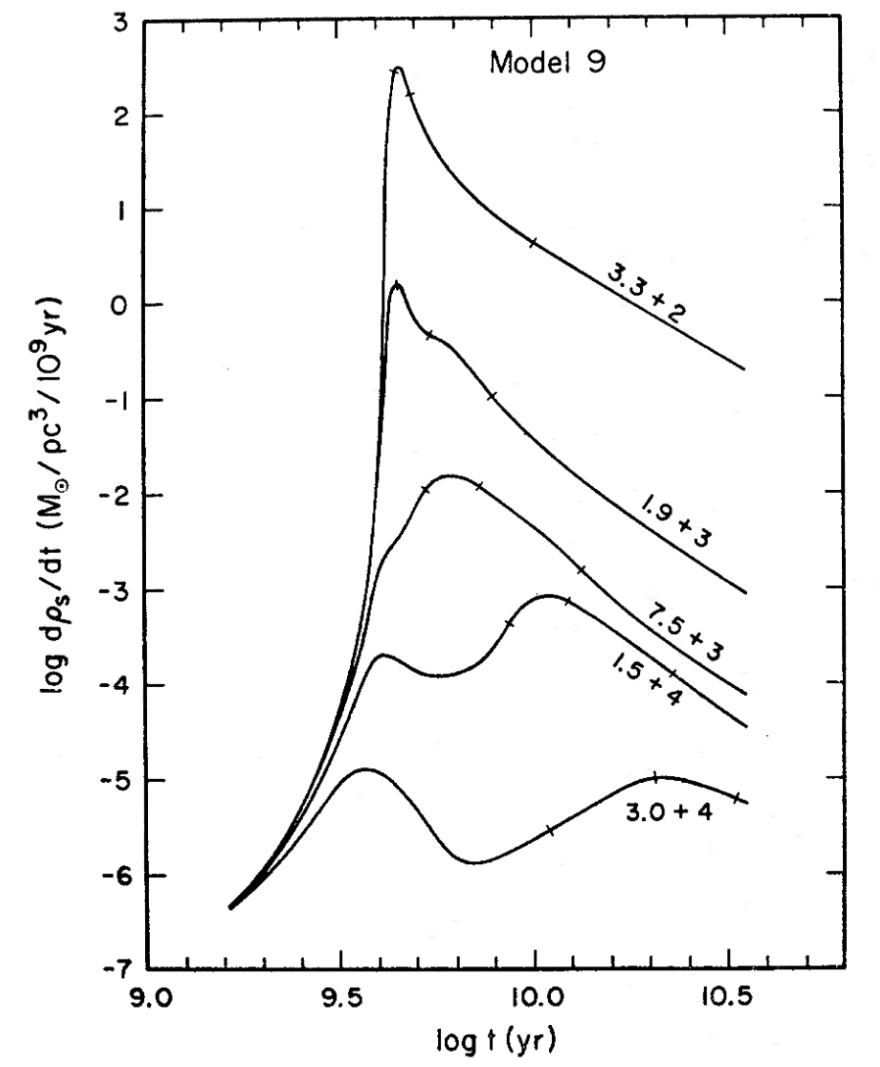
\includegraphics[width=\columnwidth]{larson1976_fig13.png}
    \caption{Figure 13 from \citet{Larson+1976}. This shows the star formation rate density as a function of time for different radii for Model 9 from the paper. Annotations indicate the radius, where for example $3.3+2$ means $3.3 \times 10^2$.}
    \label{fig:larson76}
\end{figure}

We show their modelled star formation rate density as a function of time and radius in Figure~\ref{fig:larson76}. They find that there are two distinct phases of star formation: an early burst that is centrally concentrated in the spheroidal component, and a later phase that occurs as gas settles into the plane of the disc. In particular, they note that this phase consists of ``an outward-progressing wave of star formation'' \citep{Larson+1976}. This is one of the first simulations showing a sort of ``inside-out'' growth.

They conclude that high velocity collisions between gas clouds may form spheroidal systems, whilst disc systems may form from more quiescent gas that doesn't require similar collisions. This gas settles onto the disc progressively over time, starting in the centre in which the potential is strongest and then progressing outwards.

\section{Observations}
\subsection{Evidence of inside-out growth}
Using data from 3D-HST and CANDELS Treasury surveys, \citet{vanDokkum+2013} investigated the assembly of Milky-Way-like galaxies since redshift 2.5.

They use the number density of galaxies to rank them and assume that galaxies maintain the same rank throughout cosmic time. This has been shown to be a reasonably effective way of associating progenitor galaxies with their descendants \citep{Leja+2013}. They select galaxies with stellar masses close to that of the Milky Way and use this ranking method to associate galaxies together in order to measure their evolution over time. This produces a sample of approximately 400 galaxies.

After grouping galaxies into bins of redshit, \citet{vanDokkum+2013} stack galaxies and fit them using a \citet{Sersic+1968} profile (correcting for PSF effects and bootstrapping to produce error bars). We show their estimated effective radii for galaxies of different redshifts in Figure~\ref{fig:vd}.

\begin{figure}[htb]
    \centering
    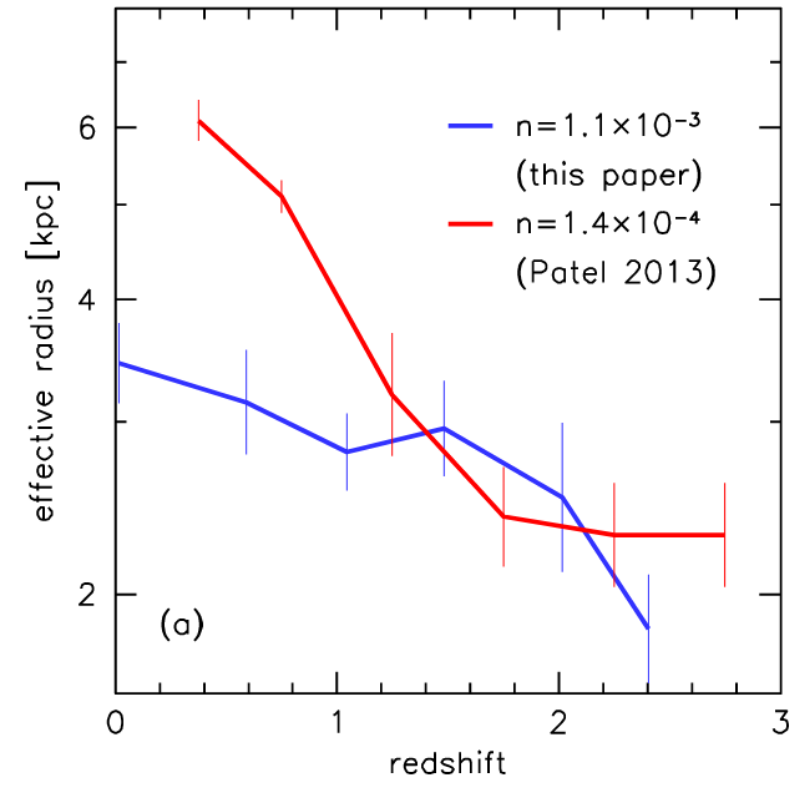
\includegraphics[width=\columnwidth]{vandokkum2013_fig5.png}
    \caption{Figure 5 from \citet{vanDokkum+2013}. The effective radius of observed galaxies from 3D-HST and CANDELS at different redshifts, compared to another paper.}
    \label{fig:vd}
\end{figure}

Figure~\ref{fig:vd} shows that the effective radius of a galaxies decreases with increasing redshift, implying that galaxies are growing over time and thus providing evidence for some sort of inside-out growth. It is also notable that within this figure they also compare to \citet{Patel+2013}, a paper that finds stronger evidence of inside-out growth in more massive galaxies. They conclude that there is likely some sort of mass dependence to the rate of inside-out growth and that galaxy formation models will need to explain both effects.

\clearpage

\subsection{A lack of strong evidence}

\begin{figure*}[t]
    \centering
    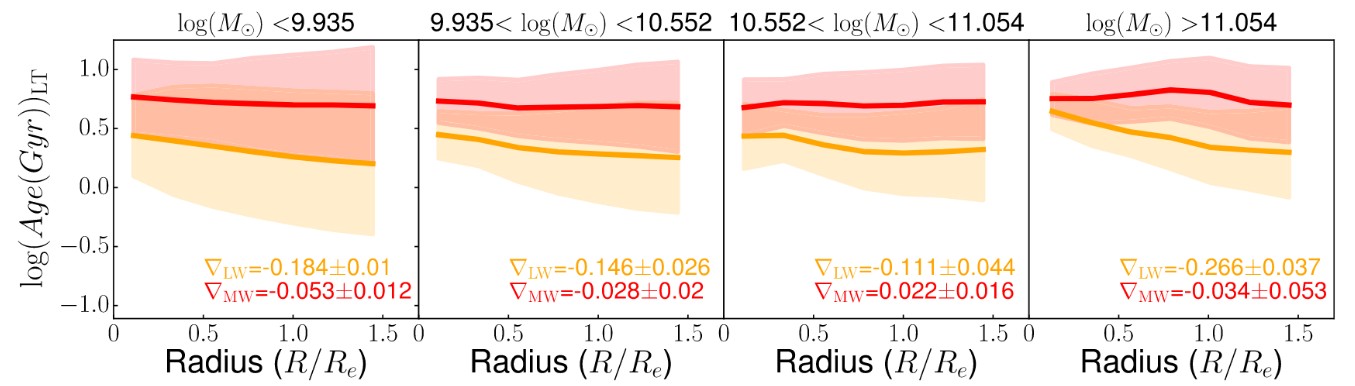
\includegraphics[width=\textwidth]{goddard2017_fig14.png}
    \caption{Figure 14 from \citet{Goddard+2017}. Mass weighted age-radius gradients are given in red for four different mass bins, from observations in SDSS-IV MaNGA.}
    \label{fig:goddard}
\end{figure*}

More recently, \citet{Goddard+2017} studied the star formation of histories in galaxies as a function of galaxy mass and type using the SDSS-IV MaNGA survey.

They selected an initial sample of 806 galaxies from the SDSS DR13 release based on whether they were part of Primary sample of MaNGA and absolute magnitude. They use \texttt{FIREFLY} to perform full spectral fitting and cross match with the Galaxy Zoo to establish the morphological classification of the galaxies. Only galaxies with an 80\% majority vote for a certain morphological type were included in the final sample to avoid irregularities. Finally, galaxies with poor velocity dispersion estimates were exluded since they resulted in poor spectral fits. This left a sample of 791 galaxies, of which 216 are spiral galaxies.

\citet{Goddard+2017} use a method of full spectral fitting to spatially resolve the age, metallicity and dust attenuation radial gradients for individual galaxies with the code \texttt{FIREFLY}. They argue that their code improves upon existing codes such as \texttt{STARLIGHT} \citep{CidFernandes+2005}, due to parameter free estimation of dust which requires no dust reddening law and improved underlying stellar tracks. They also check that beam smearing is not a significant effect through comparison with the secondary sample when restricting it to equivalent effective radii. They find that the effect of beam smearing must be quite small and does not affect the gradients in any significant way.

In Figure~\ref{fig:goddard}, we show the age-radius gradients found by \citet{Goddard+2017}. Whilst the light-weighted gradients show a very weak indication of a negative slop, the mass-weighted gradients are not statistically significant and are consistent with zero \citep[in agreement with][]{Sanchez-Blazquez+2014}. Therefore, though the light-weighted gradients show some very slight evidence for inside-out growth, the mass-weighted gradients display no such evidence.

\subsection{Why the disagreement?}
So clearly there is some tension between the results of \citet{vanDokkum+2013} and \citet{Goddard+2017} and this represents a key challenge in this topic. Both examine similar samples of galaxies and yet find very different results, indicating that either (1) one of the papers has an error in their analysis or (2) there is another effect at play which is making a difference between the two samples.

With that in mind, we can now consider some recent models for inside-out growth that include a provision for radial migration as a potential solution for this tension.

\section{A model for inside-out growth}
\citet{Frankel+2019} made a key development in this area by creating and applying a framework for a global evolution Milky Way disc model with an emphasis on inside-out growth. They note the observational tension and highlight that the importance of dynamical heating from spiral arms and molecular clouds has long been recognised and should be accounted for. They point out that observations are restricted to studying present-day radii of stellar populations rather than their unknown birth sites and this has a strong effect on the observed gradients.

They argue that, given that we have access to positions, chemical compositions and ages of \textit{individual} stars in the Milky Way, we may be able to trace their birth positions through weak chemical tagging and fit a model for inside-out growth and radial migration simulataneously.

With this goal in mind, they attain a sample of around 5000 red clump giant stars from APOGEE that have asteroseismically calibrated ages, metallicities and 3D positions. These stars in particular were chosen since they have similar core mass and therefore similar luminosities, which makes them useful standard candles. They also focus only on the low-$\alpha$ disc to avoid undesired information from older stars. This means the model mainly describes the recent evolution of the outer disc.

\citet{Frankel+2019} model a variety of effects and have distributions for star formation rates, surface densities and metallicities. We focus in particular in their models for inside-out growth and radial migration. They state that the star formation history is a function of age $\tau$ as
\begin{equation}
    \text{SFH} \propto \exp \qty[ \frac{1}{\tau_{\rm sfr}} \qty( \qty[1 - x \frac{R_0}{8 \unit{kpc}}] \tau - \tau_m ) ],
\end{equation}
where the inside-out growth is encoded in the dimensionless parameter $x$ ($\tau_{\rm sfr}, \tau_m$ are other parameters of the model that are fit for and $R_0$ is the birth radius). From this equation we can see that a value of $x > 0$ would imply inside-out growth, whilst $x < 0$ is outside-in and $x = 0$ means constant formation across the disc.

\begin{figure}[b]
    \centering
    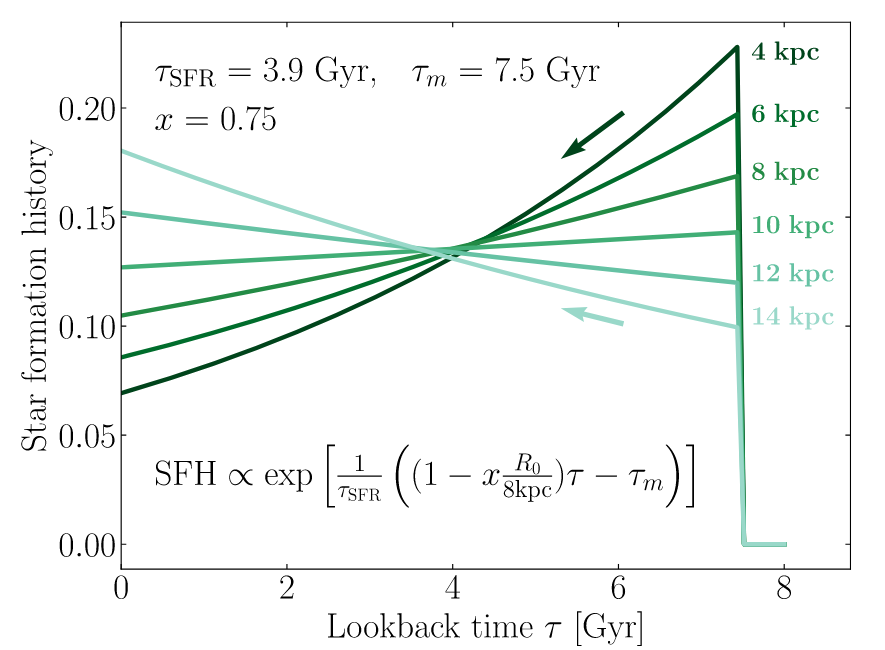
\includegraphics[width=\columnwidth]{frankel2019_fig5.png}
    \caption{\citet{Frankel+2019} Figure 5 showing the model for inside-out growth with the best fit set of parameters (values are annotated).}
    \label{fig:frankel_io_model}
\end{figure}

This equation is plotted in Figure~\ref{fig:frankel_io_model} for the best fit set of parameters which demonstrate inside-out growth. One can see that formation for small radii peaks at small radii, whereas formation as large radii is still increasing at present day.

For radial migration, \citet{Frankel+2019} define the probability that a star is found at a radius $R$ given that it was born at a radius $R_0$ at a time $\tau$ as
\begin{equation}
    p(R | R_0, \tau) \propto \exp \qty(- \frac{(R - R_0)^2}{2 \sigma_{\rm RM7}^2 \qty(\frac{\tau}{7 \unit{Gyr}})}),
\end{equation}
where $\sigma_{\rm RM7}$ is a constant that defines the global diffusion strength of radial migration.

\begin{figure}[tb]
    \centering
    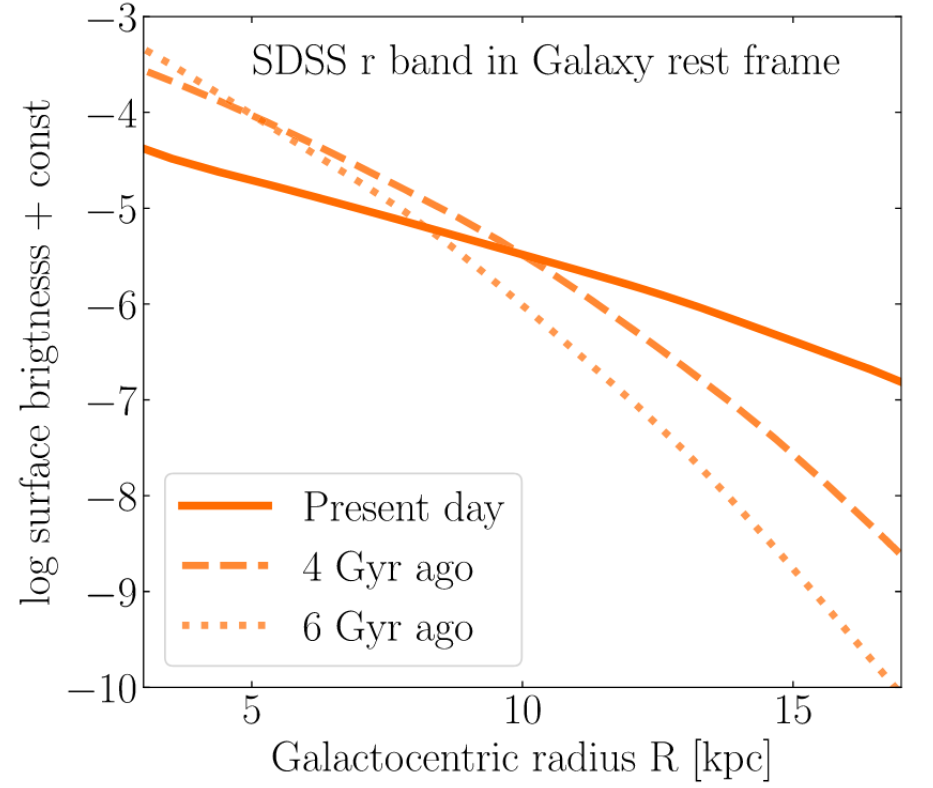
\includegraphics[width=\columnwidth]{frankel2019_fig9.png}
    \caption{\citet{Frankel+2019} Figure 9. Mock observations of what SDSS would observe for the Milky Way's surface brightness profile when observed at different times. Each line represents an observation at a different points in time.}
    \label{fig:frankel_sdss}
\end{figure}

After fitting for these two distributions and several others, \citet{Frankel+2019} find a best fit to the Milky Way's low-$\alpha$ disc as $x = 0.75$, implying that inside-growth has occured within the Milky Way disc. It indicates that star formation has been constant at a radius of around $10.5 \unit{kpc}$, decreasing within this radius and increasing outside of it. They also find that the radial migration strength is much strong than zero with a value of $\sigma_{\rm RM7} = 3.9 \unit{kpc}$, which (I \textit{think}) means that stars that formed 7 Gyr ago will on average move by nearly 4 kpc.

They present these results as a resolution of the tension among different observations. The lack of evidence could be interpreted as a lack of inside-out growth, however \citet{Frankel+2019} argue that it is instead evidence of wide-scale radial migration erasing traces of inside-out growth over time. In Figure~\ref{fig:frankel_sdss}, we show their predictions for what SDSS would observe when looking at the Milky Way a different times. The evidence of inside-out growth is clear in these observations, as older observations have a sufrace brightness profile more clearly peaked at lower radii.

\begin{figure}[tb]
    \centering
    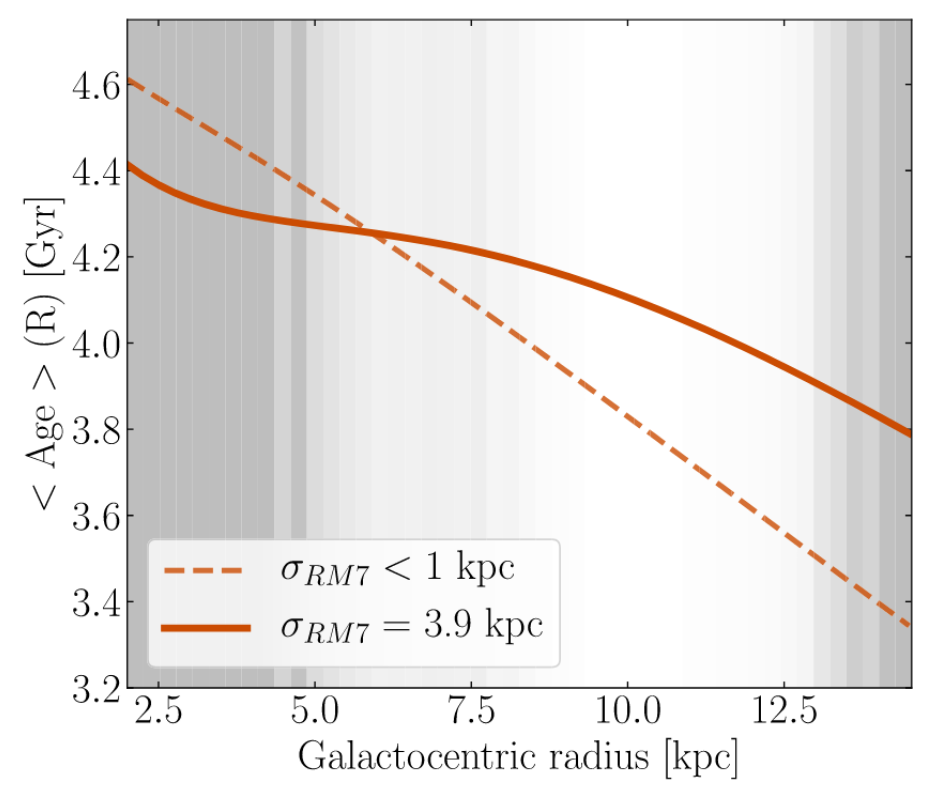
\includegraphics[width=\columnwidth]{frankel2019_fig12.png}
    \caption{\citet{Frankel+2019} Figure 12. Mass-weighted age-radius relations for the Milky Way in two cases: one with no radial migration and one with radial migration (using the best fit model from \citet{Frankel+2019}).}
    \label{fig:frankel_gradient}
\end{figure}

\citet{Frankel+2019} address the weak age gradients found in \citet{Goddard+2017} by highlighting that the effect of radial migration. In Figure~\ref{fig:frankel_gradient}, they show the mass-weighted age-radius gradient weakens in the case in which you apply radial migration (the solid orange line). This indicates that in other galaxies (many of which were observed my MaNGA), radial migration could be having an even stronger effect and erasing the inside-out evidence even further than what we see in the Milky Way. Expectations for evidence of inside-out growth should therefore be tempered by the knowledge that radial migration may severely weaken the age radius gradient over time.

\section{Applications}
An interesting result applying inside-out growth is presented in \citet{Banerjee+2020}. In this paper they show that inside-out growth is the missing link for getting NSNS (neutron star-neutron star) mergers to reproduce the observed decreasing trend of [Eu/Fe] with [Fe/H] in the solar neighbourhood without any changes to the delay time distribution or additional $r$-process sources.

NSNSs are thought to be a strong source of $r$-process enrichment within the galaxy and, in particular, their strong natal kicks can spread this enrichment to new regions from where they formed. This paper aims to reproduce the distribution of [Eu/Fe] to [Fe/H] in the solar neighbourhood using NSNS mergers alone. They create a model that accounts for the natal kick of NSs, a variety of potential delay time distributions and, critically, inside-out growth.

\begin{figure}[htb]
    \centering
    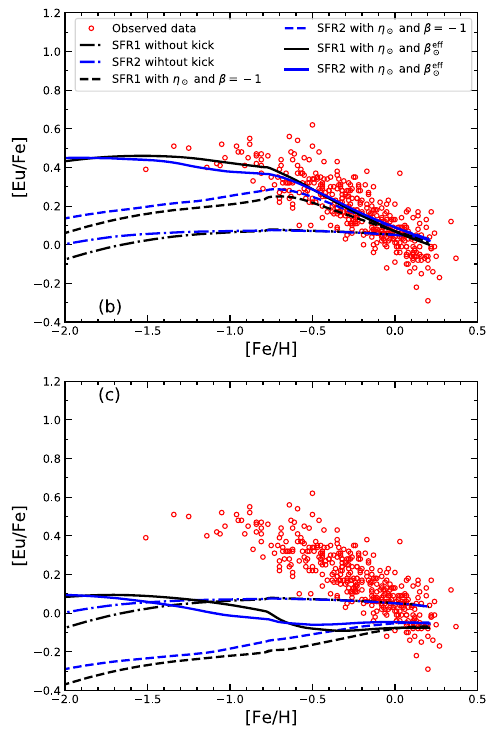
\includegraphics[width=\columnwidth]{banerjee2020_fig2.png}
    \caption{\citet{Banerjee+2020} Figure 2. Fits to the distribution of [Eu/Fe] to [Fe/H] for a series of models. The top panel uses a model including radial migration, the bottom panel assumes a fixed scale length.}
    \label{fig:nsns}
\end{figure}

In Figure~\ref{fig:nsns}, we show their results for two different models. In the top panel, NSNSs are formed at locations that account for the effect of inside-out growth, whereas in the bottom panel NSNSs are formed according to a fixed scale length of the disc. It is clear that the model accounting for inside-out growth fits the data much better and the best fitting model within this group reproduces the distribution quite well. This is rather exciting!

I will now take a moment to dampen that excitement with some comments about their assumptions about the formation of NSNS binaries, which seem a little shaky. They assume a kick distribution following an exponential peaked around $90 \unit{km}{s^{-1}}$, whilst most papers more recently agree that the distribution should follow a double maxwellian with a peak around $30  \unit{km}{s^{-1}}$ for electron capture supernovae and a peak around $265 \unit{km}{s^{-1}}$ for core collapse supernovae. Additionally they don't seem to worry about disruptions at all (as far as I can see) and assume that there is a single kick instead of two. However each NS should get a kick, and the correlation between their directions is nontrivial when conditioning on only the surviving ones (since certain combinations of directions are more likely to result in disruptions). All that being said I may just be misunderstanding things, but this confuses me at first glance. 

\section{Future Directions}
As discussed in \citet{Frankel+2019}, the main uncertainty currently on their model for inside-out growth and radial migration comes from the poorly constrained ages of stars. An interesting future direction would be to fit this model again using a sample of stars with better constrained ages and see how this could affect the model (in particular the strength of inside-out growth and radial migration). With a data set with more precise distances like Gaia, the data selection should also be less prone to population selection effects \citep{Hogg+2019} and provide a better fit for the Milky Way.

\section{Summary}
In summary, inside-out growth is the concept that spiral galaxies form from the inside out, with star formation first occuring in the centre before progressing outwards. We discussed some of the early simulations of galaxies and how it led to the acknowledgement of the necessity of inside-out growth to reproduce disc components with significant masses \citep{Larson+1976}. We explored various observations that search for evidence of inside-out growth, consider both cases in which evidence was found using 3D-HST and CANDELS \citep{vanDokkum+2013} and cases in which there was a significant lack of evidence when considering mass-weighted age-radius gradients using SDSS-IV MaNGA \citep{Goddard+2017}. We considered a new models that includes provisions for both inside-out growth and radial migration and how it implies that weaker age gradients are a direct result of strong radial migration erasing information \citep{Frankel+2019}. Finally, we examined some more recent applications of inside-out growth to the idea of $r$-process enrichment from NSNS mergers and considered some potential future directions in this area \citep{Banerjee+2020}.

\begin{acknowledgements}
    I thank Pixar for making a cinematic masterpiece about inside-out growth (emotionally at least) that was just nearly as scintillating reading these papers. I also thank my laptop for not losing any data despite the fan malfunctioning and the whole thing nearly exploding and I thank GitHub for having my back on that just in case. Finally I also thank Jim for a great class and hope he can forgive me for the quality of this paper.
    
    Since this is acknowledgements, I will also acknowledge that this isn't my very best work, but it's been quite the quarter and I would like to sleep now and lay this to rest :D
\end{acknowledgements}

\bibliographystyle{aasjournal}
\bibliography{refs}{}

\end{document}